% CVPR 2022 Paper Template
% based on the CVPR template provided by Ming-Ming Cheng (https://github.com/MCG-NKU/CVPR_Template)
% modified and extended by Stefan Roth (stefan.roth@NOSPAMtu-darmstadt.de)

\documentclass[10pt,twocolumn,letterpaper]{article}

%%%%%%%%% PAPER TYPE  - PLEASE UPDATE FOR FINAL VERSION
%\usepackage[review]{cvpr}      % To produce the REVIEW version
\usepackage{cvpr}              % To produce the CAMERA-READY version
%\usepackage[pagenumbers]{cvpr} % To force page numbers, e.g. for an arXiv version

% Include other packages here, before hyperref.
\usepackage{graphicx}
\usepackage{amsmath}
\usepackage{amssymb}
\usepackage{booktabs}
\usepackage{graphicx}
\usepackage{caption}
\usepackage{float}
\usepackage{dblfloatfix}
\usepackage{tabularx}
\usepackage{array}
\newcolumntype{L}{>{\centering\arraybackslash}m{1.5cm}}
\newcolumntype{?}{!{\vrule width 1pt}}
\makeatletter
\def\hlinewd#1{%
\noalign{\ifnum0=`}\fi\hrule \@height #1 %
\futurelet\reserved@a\@xhline}
\makeatother


% It is strongly recommended to use hyperref, especially for the review version.
% hyperref with option pagebackref eases the reviewers' job.
% Please disable hyperref *only* if you encounter grave issues, e.g. with the
% file validation for the camera-ready version.
%
% If you comment hyperref and then uncomment it, you should delete
% ReviewTempalte.aux before re-running LaTeX.
% (Or just hit 'q' on the first LaTeX run, let it finish, and you
%  should be clear).
\usepackage[pagebackref,breaklinks,colorlinks]{hyperref}


% Support for easy cross-referencing
\usepackage[capitalize]{cleveref}
\crefname{section}{Sec.}{Secs.}
\Crefname{section}{Section}{Sections}
\Crefname{table}{Table}{Tables}
\crefname{table}{Tab.}{Tabs.}


%%%%%%%%% PAPER ID  - PLEASE UPDATE
\def\cvprPaperID{00002} % *** Enter the CVPR Paper ID here
\def\confName{CVPR}
\def\confYear{2024}


\begin{document}

%%%%%%%%% TITLE - PLEASE UPDATE
\title{A Tailored CNN for CIFAR-10: 

Leveraging Fine-Tuned VGG16, ResNet50, and EfficientNet-B0 Models}

\author{Brian Drake\\
University of Adelaide\\
THE UNIVERSITY OF ADELAIDE
5005 AUSTRALIA\\
{\tt\small brian.drake@student.adelaide.edu.au}
% For a paper whose authors are all at the same institution,
% omit the following lines up until the closing ``}''.
% Additional authors and addresses can be added with ``\and'',
% just like the second author.
% To save space, use either the email address or home page, not both
}
\maketitle

%%%%%%%%% ABSTRACT
\begin{abstract}
This study investigates the performance of Convolutional Neural Networks (CNNs) for image classification on the CIFAR-10 dataset. The models tested include a baseline initial model, as well as fine-tuned versions of ResNet50, EfficientNet B0, and VGG16. An improved model was then also developed, integrating features from the aforementioned architectures. The improved model performed the best, achieving a training accuracy of 92.77\% and a test accuracy of 79.59\%, with an error rate of 20.41\% after only 10 epochs. Training was extended to 50 and 100 epochs, leading to improvements in training accuracy, 98.82\% at 50 epochs, but a decline in test accuracy, 81.95\% at 100 epochs, indicating overfitting. Comparison with other models showed that the EfficientNet model achieved a test accuracy of 82.73\%, while ResNet50 and VGG16 demonstrated lower performance. The outcome of this study highlights the effectiveness of combining transfer learning with architectural innovations from VGG, ResNet, and EfficientNet, to develop a more efficient and accurate image classification model. While indicating room for further optimisation through regularisation techniques and hyperparameter tuning.
\end{abstract}

%%%%%%%%% BODY TEXT
\section{Introduction}
\label{sec:intro}
The CIFAR-10 (Canadian Institute for Advanced Research) dataset is a historically established computer vision dataset used for object recognition. Comprised of 60,000 32x32 pixel, colour images distributed evenly across 10 classes; airplane, automobile, bird, cat, deer, dog, frog, horse, ship, and truck. These classes are mutually exclusive and do not overlap for the purposes of object classification \cite{cifar10}. This dataset is primarily used for experiments in computer vision due to the small image sizes and simple but challenging class distinctions, for example, cat and dog and automobile and truck.

Computer vision is achieved via Convolutional Neural Networks (CNN). Using a CNN model can enable images, such as the CIFAR-10 dataset, to be identified and classified. CNNs are a specific type of multilayer neural network based on living vision. A traditional CNN is comprised of a single or even multiple blocks of these convolutional layers. The aim of these layers is to enable feature extraction, whereby a matrix of values can characterise shape, texture, pattern etc \cite{recent_trends}. Resulting in a model that can learn what categories of data "look like" and then classify them. While this is an established field in computer vision, machine learning, and artificial intelligence, problems remain in computational time, load, and accuracy. 

Breakthrough models like the VGG \cite{original_vgg}, ResNet \cite{original_resnet}, and EfficientNet \cite{original_efficientnet} families have all driven significant advancements in computer vision. These model families are widely available in libraries like PyTorch and TensorFlow. Where they can be accessed with or without pretrained weights, often from large datasets like ImageNet. ImageNet is a large and varied dataset with many images, some of which are from CIFAR-10, that are used to train deep CNNs to distinguish between 1000 object classes. Training at this scale demands substantial compute, storage, and time. However, the resulting trained model can be saved and reused through transfer learning or fine tuning. Whereby these extracted model weights can be used directly or adapted to new datasets, supporting a wide range of projects without requiring extensive resources. Leveraging the previous learning, transfer learning accelerates feature extraction and reduces training time. Through the analysis of these fine tuned models, optimisation of simpler models into tailored, deep architectures can be utilised to produce an improved model for the CIFAR-10 dataset.


\section{Method}
\label{sec:method}
A fundamental model was developed using computer vision techniques. This involved the use of multiple 2D Convolutional layers, Batch Normalisation, Max Pooling, and Dense layers, as well as the incorporation of Dropout.

Convolutional layers are a mathematical process whereby primarily image data is processed to extract features such as edges, textures, and shapes. A layer applies small filters, or kernels, which are matrices of learnable weights across the input image. Each filter slides, or convolves, across the entire image. At each position a dot product is calculated between the filter and the covered cell of the image matrix. Resulting in a single output value which forms part of the new matrix called a feature map. Multiple layers are applied to create multiple feature maps designed to capture different aspects of the input image. The output is typically passed through a non-linear activation function like ReLu. Intended to introduce non-linear learning, assisting in learning complex patterns. Further, in general the more convolution layers added to a neural network, the more complex features that network can learn. Most convolutions will require padding, padding refers to the space outside of the input matrix itself where a kernel may require data. This padded  data can be filled in, in multiple ways depending on the networks needs. A padding of "same" projects the nearest number in the matrix over the edge to reduce the impact on the convolution calculation itself \cite{convolutiontheory}. An example of this entire process can be seen in figure \ref{fig:Convolution example}, where the second cell of a 2D convolution with a 3x3 filter and 'same' padding is being applied. 

\begin{figure} [h]
    \centering
    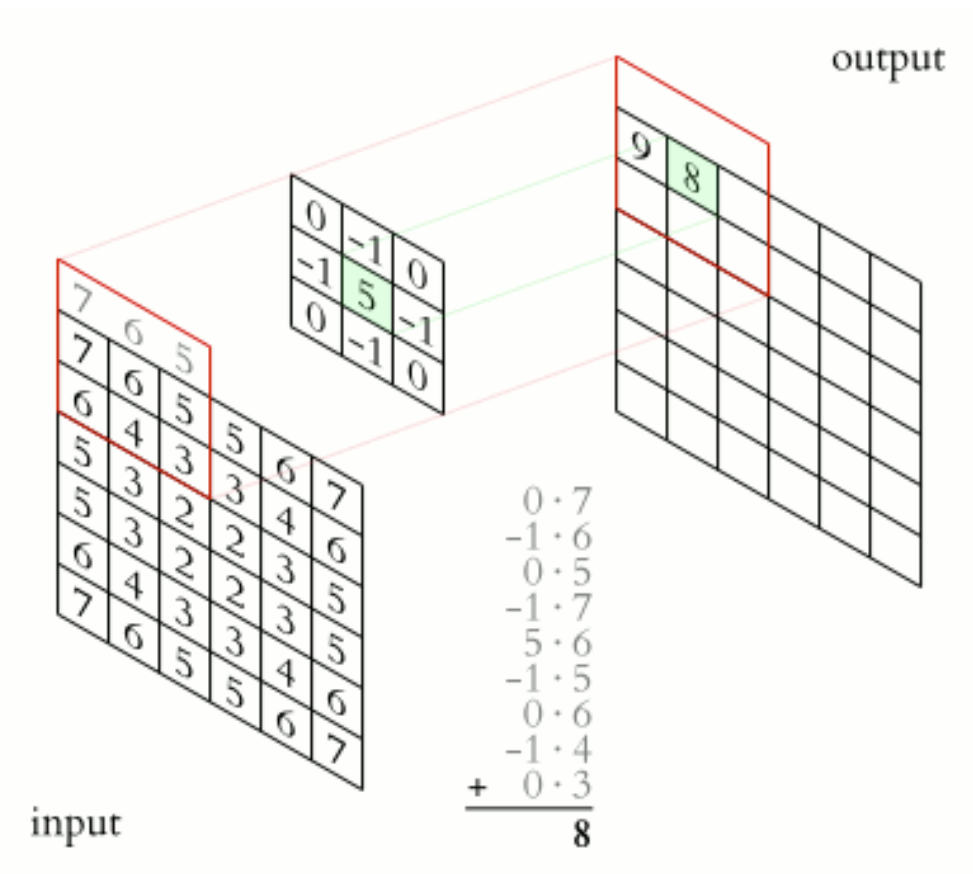
\includegraphics[width=\linewidth]{convolution.png}
    \caption{An example of a 2D convolution \cite{convolutiondiagram}}
    \label{fig:Convolution example}
\end{figure}

Batch Normalisation is a function used where inter-layer outputs of a neural network are transformed to maintain a mean of approximately 0 and a standard deviation of approximately 1 \cite{pytorch}. Enabling faster computation due to the outputs being scaled to a smaller set of numbers. Combating the exploding gradient problem and enabling epochs to resolve faster, due tot he smaller computational load. This is represented mathematically as:

\[y = \frac{x-E[x]}{\sqrt{Var[x]+\epsilon}} * \gamma + \beta\]

Where the mean and standard deviation are calculated per-dimension, with \(\gamma\) and \(\beta\) being learnable parameter vectors of size C. Where C is equal to the number of features or channels of the input.

Max Pooling is a down sampling layer used within CNNs. This reduces spatial dimensions (width and height) of the input feature maps, while retaining the most important information. This operation works similarly to a convolution where a kernel is slid over the matrix but instead of summing the convolution into a single cell, the maximum value is taken within that region and used. Allowing the network to retain critical information about features while reducing computational load \cite{recent_trends}. By reducing the spatial size and therefore the resolution of the feature map the model becomes more robust toward small translations or distortions in the input data. In tandem max pooling acts as a form of regularisation and mitigates some overfitting. 

A dense layer, or fully connected layer, is a layer in a neural network where each neuron connects to every neuron in the preceding layer. This structure enables dense layers to integrate information learned from previous layers and form complex pattern recognition. Each neuron in a dense layer has an associated weight and activation function, allowing data transformation and interpretation \cite{pytorch}. Learning nonlinear relationships that contribute to the network's predictive capabilities. Dense layers are typically used in the final stages of a CNN to output predictions or classifications based on the learning achieved. 

Dropout is a functional layer used during training of a neural network where some elements of the input tensor are randomly changed to zeroes. Achieved as an independent probability, as specified in the architecture itself, that each node is changed \cite{pytorch}. Depending on the model not only can different probabilities be passed but multiple occurrences of dropout can be used. Dropout is intended to improve regularisation by preventing the co-adaptation of individual nodes \cite{hinton2012improvingneuralnetworkspreventing}. Meaning that increased complexity of the model will be less likely to create redundant or silent nodes. In turn allowing for greater generalisation on new data. 

\subsection{VGG16}
VGG16 is one of a family of deep convolutional neural networks created by the Visual Geometry Group (VGG) at Oxford. It is characteristic of having 16 layers, 13 convolutional and 3 fully connected. The constituent convolutional layers use a 3x3 kernel with a stride of 1 and 'same' padding to maintain spatial resolution. VGG16 also stacks multiple convolutional layers, 2-3 consecutively, followed by a max pooling layer. Until finally the network ends with three fully connected perceptron layers, purposed to handle high level feature data extracted by the previous layers \cite{original_vgg}. This is a straight forward architecture that can extract features but due to its depth and fully connected layers requires large computational input, memory, and requires a strict learning rate when training. 

\subsection{ResNet50}
ResNet50 is the 50 layer version of the ResNet (Residual network) deep convolutional neural network family of models. Originally introducing residual learning to address the vanishing gradient problems that have arisen alongside deep networks. ResNet's contribution to computer vision is the unique residual connections they contain, which allow learning from "residual" functions rather than trying to learn from the full feature mapping. Allowing for simplification of optimising deep networks. This is achieved by taking an initial convolution before the convolution block begins then adding those back at the end of the block. Creating a shortcut for the block in feature extraction. The 50 layer architecture also featured a bottleneck design where the kernel will be 1x1 then 3x3 then 1x1 again in a convolution block, rather than one consistent size. Further, instead of multiple dense layers, ResNet uses a global average pooling and a single dense layer, to further reduce computational parameters \cite{original_resnet} \cite{finetuningresnet50}. Thus enabling ResNet50 to be highly efficient and maintain accuracy even in deep architectures. The key drawbacks however, are the requirement for careful implementation and interpretation. 

\subsection{EfficientNet}
EfficientNet is a family of models designed around the use of a compound scaling method to balance depth, width and resolution of a neural network. Achieving higher accuracy with fewer parameters. The chosen EfficientNet model was B0, the simplest and first of the family. Presenting the Inverted Bottleneck Block where, similar to MobileNetV2 and ResNet, the convolution blocks start at smaller kernels then increase before dropping off again. For example central 7 blocks kernels are in order 3x3, 5x5, 5x5, and lastly a 3x3, format. Creating a tight bottle neck when data enters and exits rather than building a larger and larger or static kernel size as the model deepens. Creating "Squeeze and Excitation" layers that re-weight channel wise feature maps \cite{original_efficientnet} \cite{fintuningefficientnet}. The resultant architecture creates a high accuracy model with fewer parameters. Forming a desirable model for resource limited environments. The key drawback to this approach is fact that more tuning is required to achieve optimal performance.

\subsection{Performance Metrics}
The performance of all models will be assessed via three helper functions. Where the confusion matrix, loss over epochs, accuracy over epochs, test accuracy, and test error rate can be discerned. The confusion matrix provides data on how the model is predicting newly presented data, assisting in the identification of underfitting, overfitting, uneven class representation, and confounding class feature extraction. The contusion matrix performance ideally should be comparable to model accuracy. The loss over epochs and accuracy over epochs metrics provide insight into model convergence and model performance, allowing for assessment of underfitting and overfitting. Finally test accuracy and test error rate enable an overview of the models performance on unseen data, providing insight on the models ability to generalise. This is achieved when comparing the models reported accuracy to the test accuracy, characterised against test error rate. Where a high model accuracy, high test accuracy, and low error rate are indicative of an optimal model. 

\begin{table*}[!ht]
\centering
\begin{tabular}{?L?L?L?L?L?L?L?L?L?}
\hlinewd{1pt}
\textbf{Model} & \textbf{Parameters (Million)} & \textbf{Epochs} & \textbf{Training Accuracy (\%)} & \textbf{Test Accuracy (\%)} & \textbf{Test Error (\%)} & \textbf{Average Epoch Time (seconds)} & \textbf{Fine Tuned} & \textbf{Confusion Matrix Reflective} \\ \hlinewd{1.5pt}
ResNet50 & 48.8 & 10 & 76.95 & 67.13 & 32.87 & 87.5 & Y & Y \\ \hline
EfficientNet & 26.1 & 10 & 86.67 & 82.73 & 17.27 & 53.2 & Y & Y \\ \hline
VGG16 & 33.6 & 10 & 9.73 & 10.00 & 90.00 & 71.3 & Y & Y \\ \hline
Initial Model & 19.0 & 10 & 91.83 & 76.84 & 23.16 & 20.5 & N & Y \\ \hline
Improved Model & 5.39 & 10 & 92.77 & 79.59 & 20.41 & 37.0 & N & Y \\ \hline
Improved Model & 5.39 & 50 & 98.29 & 82.98 & 17.02 & N/A & N & Y \\ \hline
Improved Model & 5.39 & 100 & 98.82 & 81.95 & 18.05 & N/A & N & Y \\ \hlinewd{1pt}
\end{tabular}
\caption{Performance comparison of all models}
\label{tab:model_performance}
\end{table*}

\section{Experimental Analysis}
\label{sec:expana}
The CIFAR-10 dataset was provided by TensorFlow using the tensorflow.keras.datasets.cifar10 function. The dataset was imported in an already split format, 5:1 (train:test). The imported data was then checked for shape and size to ensure it was imported correctly before the images were flattened into individual matrices. They were then visualised to check that the classes were correct and balanced. After which the individually flattened image matrices were reshaped to be compatible with training, and the channels normalised to prevent colour based bias. Finally, the true labels were then one hot encoded. 

Three helper functions were developed to test the performance of each model. The confusion\_matrix function, plots a confusion matrix for the passed model, test data, and test label variables. Achieved via the TensorFlow library's confusion matrix function. The plot\_performance helper function plots the training losses and accuracy independently over epochs from the passed model's history object. Finally, the test\_error function calculates the test accuracy and error rate of the passed model against the test data; printing the outcome as a statement, including the percentage rounded to 2 decimals. 

All models were trained for 10 epochs. The final improved model was the only model to be further trained until 50 and then 100 epoch thresholds. All fine tuned models were imported without top layers, unfrozen deep layers, and identical custom top layers. This custom top layer was also used for the final portion of the initial model. All models were compiled using the Adam optimiser set to default options, categorical cross entropy loss calculations, and the accuracy metric output for each epoch step. These design decisions and constraints were made to enable the most comparable architectural results between all models. The measured metrics and some additional data was tabulated into table \ref{tab:model_performance}. 

The initially designed model for optimisation was developed using traditional CNN architecture. It was consistent of three convolutional blocks, made of two 2D convolutional layers followed by Batch Normalisation and then 2D Max Pooling (with a 2x2 kernel). These blocks were arranged consecutively in increasing convolutional size (64, 128, 512), with a static 3x3 kernel and "same" padding. The resulting feature maps were flattened before being fed forward to the top layers of the model. The top layers were consistent between the initial and fine tuned models. Constituent of a 4096 dense layer with 30\% dropout, then another 4096 dense layer without dropout. Ultimately outputting to a 10x1 softmax matrix. 

The resultant initial model presented a 91.83\% accuracy corroborated with a 76.84\% test accuracy and error rate of 23.16\%. This was meaningfully reflected in the confusion matrix with some difficulties differentiating between birds, cats, dogs, and deer. The losses and accuracy over epochs suggests that the model is nearing convergence after the 10 epoch. Due to the shallow nature of this initial model in comparison to the newer models, the average epoch training time was 20.5 seconds. This performance reflects the more shallow architecture as the model is able to perform well with low dimensional image data. Enabling the high training accuracy, fast convergence, and quick descent to overfitting. 

\begin{figure*}[ht]
    \centering
    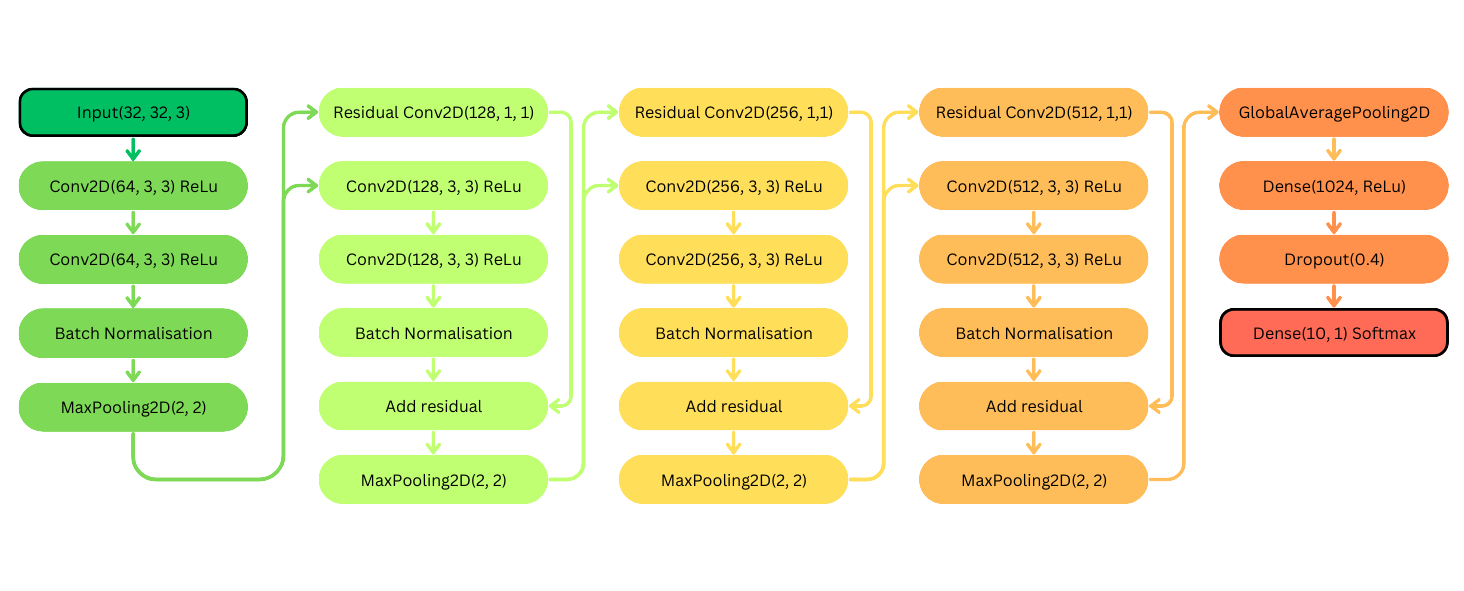
\includegraphics[width=1 \textwidth, height=0.31 \textheight]{Improved Model Flowchart.png}
    \caption{Structural Flowchart of the Improved Model}
    \label{fig:improved model}
\end{figure*}

\subsection{Fine Tuned Models}
The ResNet50 model was fine tuned with the initial weights imported from TensorFlow after training on the ImageNet dataset. After 10 epochs the model presented a 76.95\% accuracy with an average 87.5 seconds per epoch time. The test accuracy was 67.13\% and the error rate a reciprocal 32.87\%. The confusion matrix meaningfully reflected this performance, consistently across all categories. The classes truck, ship and airplane being the easiest for the model to discern. The accuracy and losses over epochs indicate that the model is needing additional epochs for convergence but confirm that learning has meaningfully occurred.

The EfficientNet model was fine tuned with the initial weights imported from TensorFlow after training on the ImageNet dataset. After 10 epochs the model displayed an 86.67\% training accuracy and an average 53.2 second epoch time. The testing accuracy was a reflective 82.73\% with reciprocal error rate of 17.27\%. The confusion matrix also reflects the accuracy achieved, displaying only a difficulty in differentiating cats from dogs. The accuracy and losses over epochs display a trend that the model is approaching convergence after the 10 epochs with meaningful learning. 

The VGG16 model was fine tuned with the initial weights imported from TensorFlow after training on the ImageNet dataset. After 10 epochs the model displayed a 9.73\% accuracy, alongside a test accuracy of 10.0\% and a error rate of 90.0\%. The average time for an epoch to complete was 71.3 seconds. The confusion matrix characterises that the model has not been able to extract any features over 10 epochs. Resulting in the model is guessing that all inputs are a ship. The loss over epochs graph indicates that the model has entered a local minima and would require a smaller learning rate with additional epochs to be able to converge. This is supported by the accuracy over epochs data. 

\subsection{Improved Model}
The improved model was developed to take advantage of all the architectures presented within ResNet, VGG, and EfficientNet, by incorporating them into the initial model. The implementation of such can be seen in figure \ref{fig:improved model}. From the ResNet architecture, residual calculations were implemented surrounding each convolutional block, while global average pooling was implemented in the top layers. Additional convolutional layers at larger depths were also adapted from the VGG architecture. While included convolutional layer sizes were tempered, after consideration from EfficientNet and VGG, to reduce parameter size for efficient training. The key feature of squeeze and excite blocks from EfficientNet were not integrated due to CIFAR-10's dataset containing 32x32 pixel images. This size causes low complexity within the image itself, due to the low resolution. Meaning that additional channel attention may not be advantageous, more so when considering the channels have been normalised before model input. Further to this, due to the dataset containing 10 categories, squeeze and excite layers would be inappropriate, their inclusion leading to increased parameters, overfitting, and model instability. Therefore the improved model's total parameters have also decreased from the initial model, lowering from approximately 19.0 million parameters to approximately 5.39 million parameters. Additionally, the improved model boasts having one fifth the amount of parameters as the next smallest fine tuned model. 

The improved model was trained for 10 epochs, achieving a 92.77\% accuracy contrasted with a test accuracy of 79.59\% and an error rate of 20.41\%. The average epoch training time was an increased 37 seconds from the initial model's 20.5 seconds. The test accuracy and error rates were reflected in the confusion matrix, where differentiating dogs from cats and deer from horses remains difficult. The accuracy and losses over epochs, both display an the models approach toward convergence.

The improved model was then trained to 50 epochs, where the accuracy increased to a  98.29\% accuracy, contrasted against an 82.98\% test accuracy with an error rate of 17.02\%. The confusion matrix displays a similar but improved predictive behaviour to the 10 epoch version. Where there is still some difficulty in differentiating cats from dogs. The accuracy and losses over epochs data reveals that the model converged between 40 and 50 epochs. This can be observed by the oscillation occurring in both resultant graphs.

The improved model was then trained until 100 epochs. This model displays that convergence has indeed occurred and additional epochs has not caused any meaningful improvement. The accuracy has increased from that of the 50 epoch model, a 98.82\%, however the model also displays a decreased test accuracy of 81.95\%. This reduced performance is supported further by the increased test error rate of 18.05\% and reflective confusion matrix performance. The accuracy and losses over epochs graphs corroborate this with oscillation and marginal improvements in both categories. Indicating that overfitting is occurring.

\section{Code}
\label{sec:code}
Please find the code \href{https://github.com/Drackonack/DLF_Assignment_02}{here}.

\section{Conclusion}
\label{sec:conclusion}
This study demonstrates the potential of leveraging transfer learning and architectural understanding to improve model performance on the CIFAR-10 dataset. By analysing both the architecture and performance of fine tuned established CNN architectures, VGG, ResNet, and EffecientNet, an improved and bespoke model was developed. 

As detailed in the results, the improved model showed remarkable progress over the initial model. After just 10 epochs, the improved model achieved 92.77\% training accuracy and 79.59\% test accuracy, with an error rate of 20.41\%. Although the improved model had fewer parameters the model took longer per epoch to train due to its increased depth and complexity, creating a 37 second training epoch time. Extending training to 50 epochs improved test accuracy to 82.98\% and test error rate to 17.02\%. However, after 100 epochs, the model’s accuracy increased to 98.82\%, but decreased test accuracy to 81.95\%, highlighting the model's previous convergence and current overfitting.

In comparison, the EfficientNet model displayed strong performance, with a test accuracy of 82.73\% and a relatively low error rate of 17.27\% after 10 epochs. ResNet50 displayed middling performance after 10 epochs, with a test accuracy of 67.13\%, though its higher parameter count and longer training time suggest opportunities for optimization. The VGG16 model performed poorly, with a test accuracy near 10\%, revealing the need for the model to be configured further for meaningful performance. This was considered out of scope for the practice of the comparative study.

Overall, the improved model, drawing inspiration from the other more advanced architectures, outperformed both the intial and fine-tuned models in key metrics, demonstrating that combining strategies from VGG, ResNet, and EfficientNet offers promising results in image classification tasks. Despite the EfficientNet fine tuned model displaying a better error rate after 10 epochs, it did siaply a lower model accuracy and higher training time. The improved model also outperforms the original model developed for the CIFAR-10 dataset \cite{cifar10} achieving a 17.02\% error rate, an 0.98\% improvement in comparison to the 18\% error rate without data augmentation.

The improved model, however, would benefit from further exploration of regularisation methods or even hyperparameter tuning to ensure consistent performance across both training and test datasets. As evidenced by the decrease in test accuracy with longer training. 

The confusion matrices highlighted persistent challenges in distinguishing between certain classes, such as cats and dogs, suggesting that future work could further focus on incorporating additional feature extraction techniques. Additionally, exploring ensemble techniques or more advanced optimization strategies could help mitigate the performance drop observed at higher epochs, ensuring the model's robustness in real-world applications.


%-------------------------------------------------------------------------

%%%%%%%%% REFERENCES
{\small
\bibliographystyle{ieee_fullname}
\bibliography{egbib}
}

\end{document}